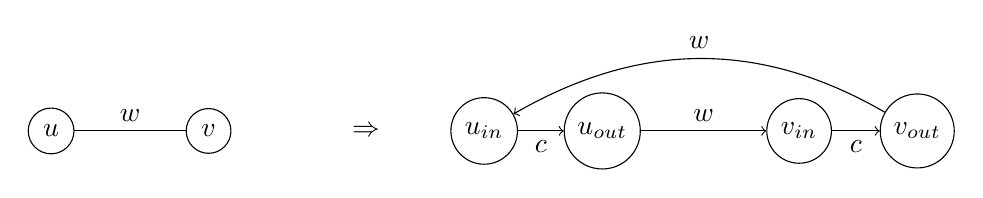
\begin{tikzpicture}
\tikzstyle{ver} = [circle, draw];

\node at (3.5,0) {$\Rightarrow$};

\node [ver] (v1) at (-0.5,0) {$u$};
\node [ver] (v2) at (1.5,0) {$v$};

\draw  (v1) edge node[above] {$w$} (v2);

\node [ver] (v6) at (5,0) {$u_{in}$};
\node [ver] (v3) at (6.5,0) {$u_{out}$};
\node [ver] (v4) at (9,0) {$v_{in}$};
\node [ver] (v5) at (10.5,0) {$v_{out}$};
\draw  (v3) edge[->] node[above] {$w$} (v4);
\draw[out=150,in=30]  (v5) edge[->] node[above] {$w$} (v6);
\draw  (v6) edge[->] node[below] {$c$} (v3);
\draw  (v4) edge[->] node[below] {$c$} (v5);
\end{tikzpicture}
